\section{Realtime Tracking}\label{sec:tracking}

\iffalse
intuition and story.

probabilistic perspective.

use probability theory to represent uncertainty and provide better estimation of the current state using back belief propagation.

augmented state: $\langle x,y,\theta,w,direction,pose\rangle$

illustrate how those state can be determined using APF.

Augmented particle filter algorithm, mainly describe what's new(importance weight calculation for resampling).
\fi


In the vehicle tracking problem, a vehicle's initial position and its relative movement w.r.t. each of its previous states are two fundamental issues to be concerned. The motion trajectory of a vehicle can, in principle, be computed by integrating the inertial sensor measurements over time given its initial position. However, due to noise and error accumulation during the integration, the dead-reckoned trajectories \cite{Robertson:Foot-mounted_Inertial, Woodman:Pedestrian_Localisation:Foot-mounted} diverge from the truth rapidly (the prediction error grows cubically in time). The drift incurred by the inertial movement unit of the phone will typically exceed 100 meters after one minute of operation \cite{Woodman:Pedestrian_Localisation:Foot-mounted}.

In this section, we will introduce a set of algorithms in VeLoc that are designed to simultaneously harness constraints imposed by the parking structure map and detected landmarks for localization a vehicle. Intuition and probabilistic explanation is presented in Section \ref{subsec:APF_intuition}, followed by algorithm details in Section \ref{subsec:APF_details}. Finally, Section \ref{subsec:APF_effect} describes how the algorithms are used to track vehicles in the parking lots.

\subsection{Intuition and Probabilistic Framework} \label{subsec:APF_intuition}
Although a noisy trajectory does not, by itself, reveal a vehicle's location, using the constraints imposed by the parking structure��s map and detected landmarks is able to help vehicle tracking. This is because (i) there may be only a few paths on the map that could accommodate the trajectory as shown in Figure \ref{fig_apf_intuition1}.
(ii) A detected landmark (e.g., a bump, turning or slope) can further pin down the positions where a vehicle might be (as shown in Figure \ref{fig_apf_intuition2}) since there are limited number of such landmarks on the map. Hence, using the synergy of both constraints is able to trace a vehicle more accurately (as shown in Figure \ref{fig_apf_intuition3}).



\begin{figure}[h]
      \centering
      \vspace{-2pt}
        \subfigure[Localization using constraints imposed by the map.] {
        \begin{minipage}[b]{0.5\textwidth}
        \centering
        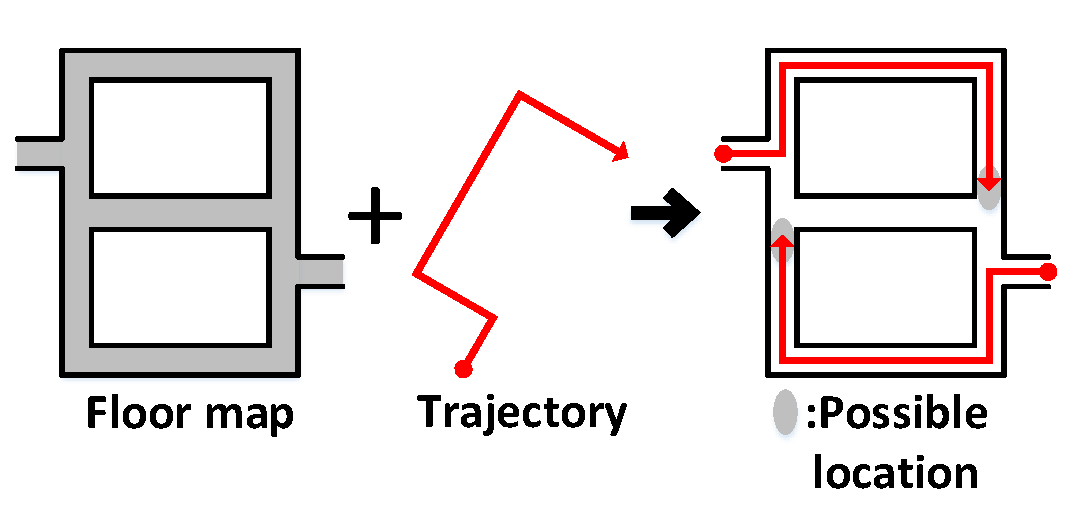
\includegraphics[width=0.9\textwidth]{apf1}\label{fig_apf_intuition1}
        \end{minipage}
        }
        \subfigure[Localization using detected landmarks.] {
        \begin{minipage}[b]{0.5\textwidth}
        \centering
        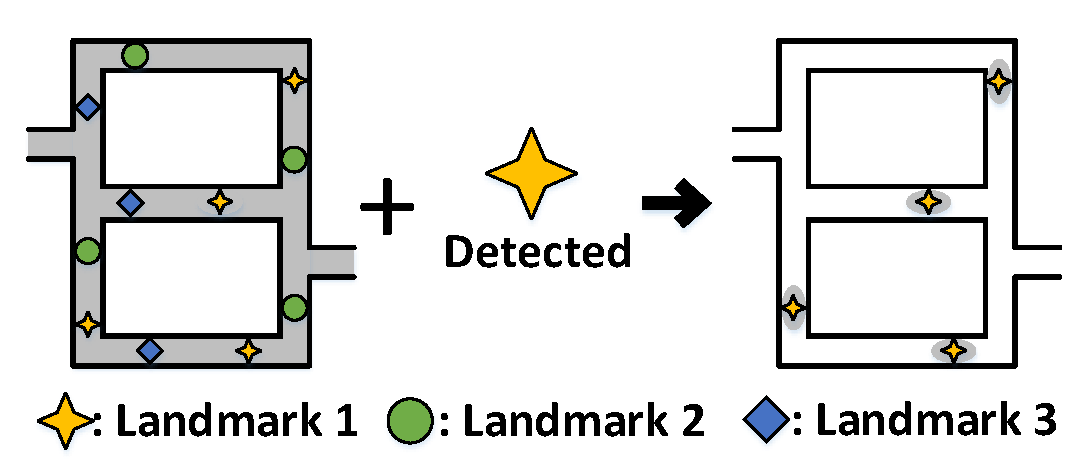
\includegraphics[width=0.9\textwidth]{apf2}\label{fig_apf_intuition2}
        \end{minipage}
        }
        \subfigure[Localization using both map constraints and detected landmarks.] {
        \begin{minipage}[b]{0.5\textwidth}
        \centering
        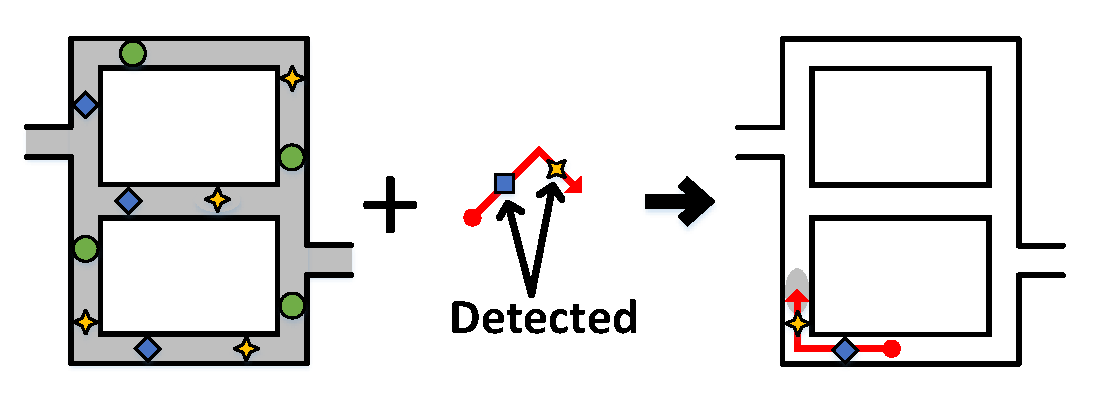
\includegraphics[width=0.9\textwidth]{apf3}\label{fig_apf_intuition3}
        \end{minipage}
        }
        \vspace{4pt}
        \caption{Intuition of localization. (a) shows that trajectories can be used for localization since only a few paths on the map could accommodate the trajectory. (b) shows that once a landmark is detected, only a few positions marked with the same kind of landmark are possible. (c) shows that using both map constraints and detected landmark could narrow down the uncertainty more quickly.}\label{fig_apf}
\end{figure}

The problem of cubically growing error in dead-reckoned trajectories \cite{Robertson:Foot-mounted_Inertial, Woodman:Pedestrian_Localisation:Foot-mounted} can also be resolved by map constraints and detected landmarks. These information provides an opportunity to re-calibrate a vehicle to correct location before the estimation error grows rapidly.

In VeLoc, we represent the uncertainty of a vehicle's states as a probability distributions over the state space. (A vehicle state includes its location, heading direction and velocity.) The tracking problem is posed as a sequential Bayesian filtering problem under the sequential importance re-sampling framework implemented by an Augmented Particle Filtering method \cite{Rai:Zee}.

We use $s_t$ to represent the state of the vehicle at time $t$, the probability distribution of vehicle states is denoted as $b(s_t)$. Bayesian filtering possesses the following two essential steps: time update and measurement update.

\textbf{Time update} is to estimate the state at time $t$ given the previous state. Different from the dead-reckoning, which simply updates the previous state with the movement, sequential Bayesian Filtering framework models the noise in movement with a probability distribution which defines the possible transitions from one state to the next as $p(s_t|s_{t-1},m_{t})$, where $m_{t}$ is the movement at time $t$.
Thus, the prior is obtained as
\begin{equation}\label{}
\overline{b}(s_t) = \int p(s_t|s_{t-1},m_{t})b(s_{t-1})ds_{t-1}.
\end{equation}

\textbf{Measurement update} is to update the probability distribution of the current state given the current measurement $m_t$. Using the Bayes rule, the posterior distribution over the state can be calculated as
\begin{equation}\label{}
b(s_t) = \eta_tp(m_t|s_t)\overline{b}(s_t),
\end{equation}
where $\eta_t$ is a normalization factor.


\subsection{Augmented Particle Filter} \label{subsec:APF_details}

Particle filter is an alternative nonparametric implementation of the sequential Bayesian filter. The key idea of the particle filter is to represent a distribution by a set of samples drawn from the distribution. The samples are called ``particles" denoted as:
\begin{equation*}
\mathcal{S}_t := \boldsymbol{s}_{t}^{(1)},...,\boldsymbol{s}_{t}^{(M)},
\end{equation*}
where M denotes the number of particles in the particle set $\mathcal{S}_t$.
Each particle $\boldsymbol{s}_t^{(i)}$($1\leq i\leq M$) is a concrete instantiation of the state at time $t$.

\textit{Augmented particles} are particles in an augmented state space. In VeLoc, the state of a particle is a five-tuple defined as $(x, y, \theta, v, d)$,
%\begin{equation*}\langle x, y, \theta, v, d\rangle\end{equation*}
where $x,y$ are position of a vehicle on a 2D floor plan, $\theta$ is the heading direction of the vehicle and $v$ is the velocity along the y-axis of the vehicle and $d$ is a binary variable, which determines the pose of the phone from two possible poses as described in Section \ref{subsec:pose_directed}.

\textbf{Time update} in our algorithm is performed by generating a hypothetical state $\boldsymbol{s}_{t}^{(m)}$ at time $t$ from its ancestor $\boldsymbol{s}_{t-1}^{(m)}$ and the current measurement $\boldsymbol{m}_t = (\omega_t, a_t)$, where $\omega$ is the rotational velocity along the z-axis of the vehicle and $a$ is the acceleration along the y-axis of the vehicle. This step involves sampling from the transition distribution $p(\boldsymbol{s}_t|\boldsymbol{s}_{t-1}, \boldsymbol{m}_t)$.
We use Gaussian distribution $\mathcal{N}(\boldsymbol{s}_t;\boldsymbol{\mu}_t, \boldsymbol{\Sigma}_t)$
to represent the transition distribution. The mean $\boldsymbol{\mu}_t$ is defined as
\begin{equation}
\boldsymbol{\mu_t} = \left(
   \begin{array}{c}
     x_{t-1} + v_{t-1}\Delta{t}\cdot\cos{\theta_{t-1}} \\
     y_{t-1} + v_{t-1}\Delta{t}\cdot\sin{\theta_{t-1}} \\
     \theta_{t-1} + \omega_t\Delta{t}\\
     v_{t-1} + a_t\Delta{t}\\
     d_{t-1} \\
   \end{array}
 \right)
\end{equation},
and $\boldsymbol{\Sigma}_t$ is diagonal matrix modeling measurement noise.

\textbf{Measurement update} in our algorithm first computes the so-called ``importance weights" (denoted as $w_{t}^{(m)}$) of each particle $\boldsymbol{s}_{t}^{(m)}$ according to $w_{t}^{(m)} \propto p(\boldsymbol{m}_t|\boldsymbol{s}_{t}^{(m)})$.
In VeLoc, the weight $w_{t}$ is computed as
\begin{equation}
w_{t} :=  \prod_{i=0}^{3}{w_{ti}},
\end{equation}
The sum of the weights at each time $t$ is normalized to one. And each $w_{ti}$ is described as follows.
\begin{itemize}
  \item \textbf{Constraints imposed by the map.} $w_{t0}$=$1$ if the position of the particle is accessible, otherwise $0$.
  \item \textbf{Detected landmarks.} For each $w_{ti}$ of the $i$-th type of landmarks ($i$=$1,2,3$), $w_{ti}$=$\mathcal{N}(D_{i}(x_t,y_t);0, \sigma_{i}^2)$ if a landmark is detected, otherwise $w_{ti}=1$. $D_{i}(x_t,y_t)$ is the distance to the closest landmark of the same type and $\sigma_{i}^2$ are parameter controlling scale of the distance.
\end{itemize}

\vspace{2mm}
The key idea of the particle filtering algorithm is \textit{sequential importance re-sampling} that draws with replacement of $M$ particles from the current set of particles according to their importance weights.
VeLoc uses Low variance sampler \cite{probabilistic} to fulfill the re-sampling task. It is worth mentioning that since re-sampling is the most time-consuming part of the algorithm, VeLoc does not perform re-sampling after every time step, instead, it maintains the importance weight for each particle, and the weights updated multiplicatively until the next re-sampling. In Veloc, re-sampling is performed every 10 time steps.


\subsection{Vehicle State Estimation} \label{subsec:APF_effect}
Using augmented particle filter as described above, VeLoc can estimate the state of the vehicle, including its location.
To illustrate how VeLoc works, we use an example scenario to drive the process of realtime tracking. Figure \ref{fig_route} shows the map of an underground parking lot with an actual route denoted by 7 key points (i.e., A to G as shown with time stamps).

\begin{figure}[htbp]
\centering
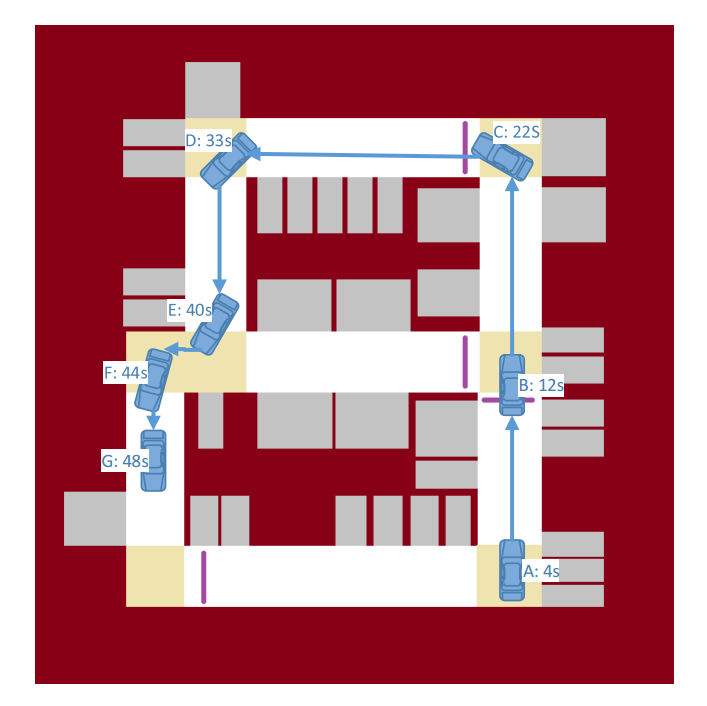
\includegraphics[scale=.3]{route.png}
\caption{Map of the example scenario shown with an actual route denoted by 7 key points and the times when the vehicle passes them. The vehicle starts at A and stops at G. }\label{fig_route}
\end{figure}

\textbf{Experiment with the initial position and heading direction of the vehicle.}
We first show in Figure \ref{fig_case1} the positions of all the particles as time goes by. Since the initial position and heading direction are known, Figure \ref{fig_case1}(a) shows that all the particles are initialized around the entrance. Figure \ref{fig_case1}(b) and (c) show that the particles diverge due to growing uncertainties caused by noises in measurements. Figure \ref{fig_case1}(d) shows that particles slightly come closer after a speed bump detection reduces the uncertainty. After a left turn, the uncertainty is greatly reduced and particles come very close (Figure \ref{fig_case1}(e)-(g)). In Figure \ref{fig_case1}(f), particles with too great or too slow speeds will hit either the front wall or side wall, and eventually disappear. Only those with appropriate speed around that of the ground truth will be able to make the left turn and continue traveling along the top isle. Figure \ref{fig_case1}(h)-(k) show how three more turns each cause more concentration of the particles. Figure \ref{fig_case1}(l) shows the final position of all the particles and the average position is shown with a red point. Compared to the actual route (Figure \ref{fig_route}), VeLocE produces a quite accurate final location.

%\begin{figure}[htbp]
\begin{figure}[t]
%\begin{tabular}{cc}
\centering
\begin{minipage}{0.32\linewidth}
  \centerline{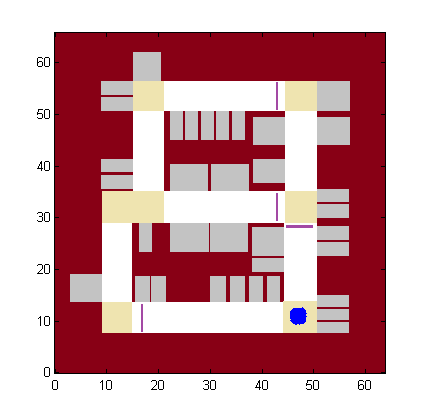
\includegraphics[scale=.3]{fig1-1.png}}
  \centerline{(a)}
\end{minipage}
\begin{minipage}{0.32\linewidth}
  \centerline{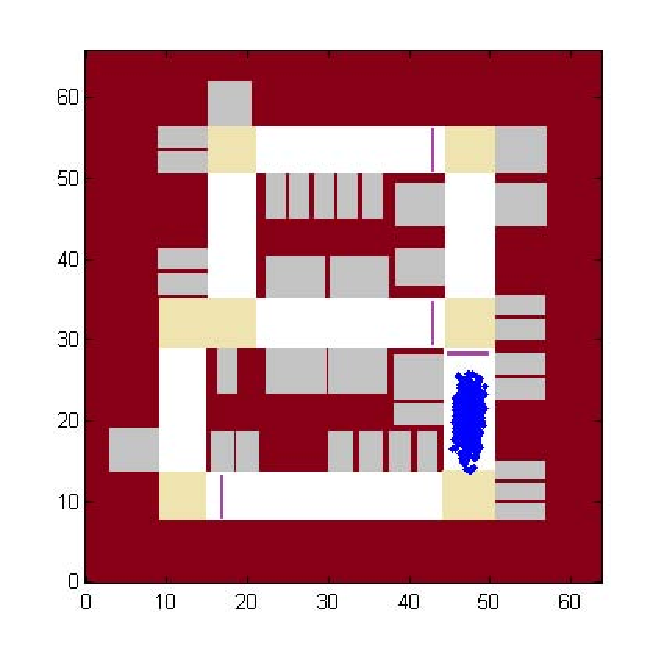
\includegraphics[scale=.3]{fig1-2.pdf}}
  \centerline{(b)}
\end{minipage}
\begin{minipage}{0.32\linewidth}
  \centerline{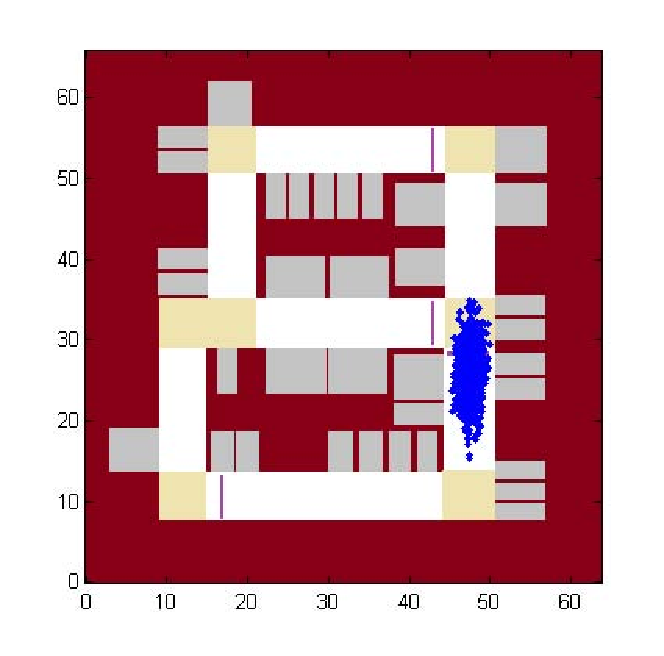
\includegraphics[scale=.3]{fig1-3.pdf}}
  \centerline{(c)}
\end{minipage}
\centering
\begin{minipage}{0.32\linewidth}
  \centerline{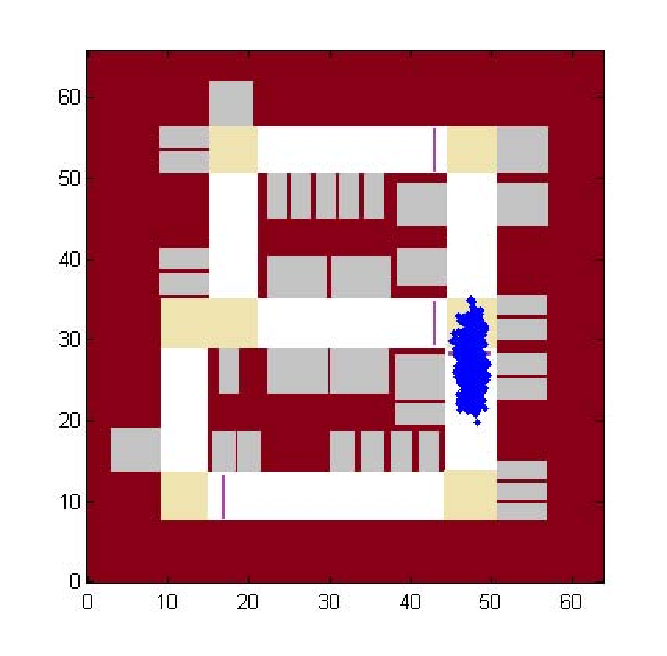
\includegraphics[scale=.3]{fig1-4.pdf}}
  \centerline{(d)}
\end{minipage}
\begin{minipage}{0.32\linewidth}
  \centerline{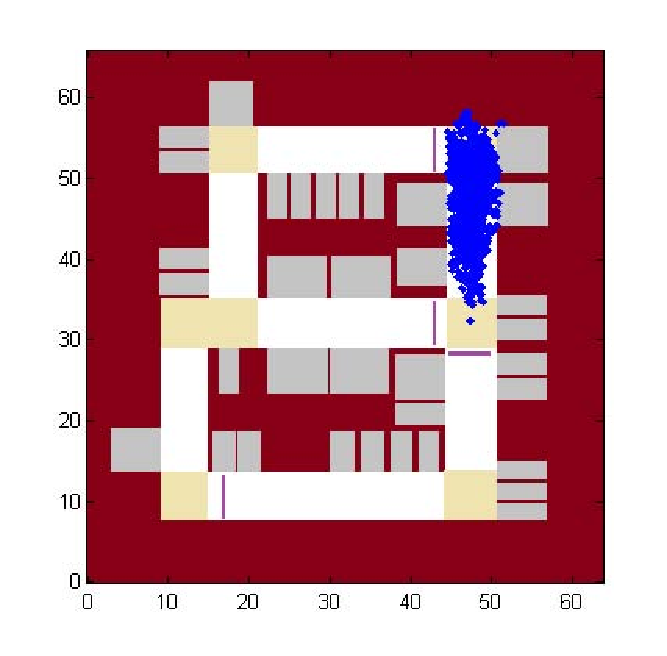
\includegraphics[scale=.3]{fig1-5.pdf}}
  \centerline{(e)}
\end{minipage}
\begin{minipage}{0.32\linewidth}
  \centerline{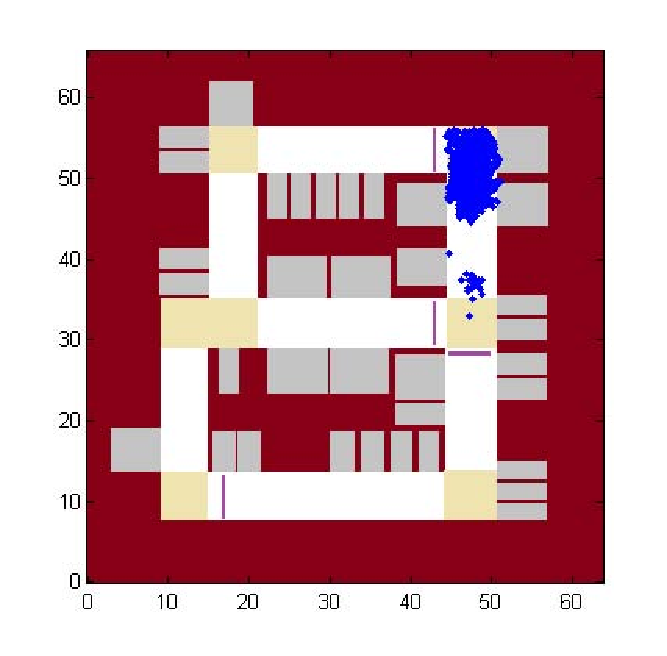
\includegraphics[scale=.3]{fig1-6.pdf}}
  \centerline{(f)}
\end{minipage}
\centering
\begin{minipage}{0.32\linewidth}
  \centerline{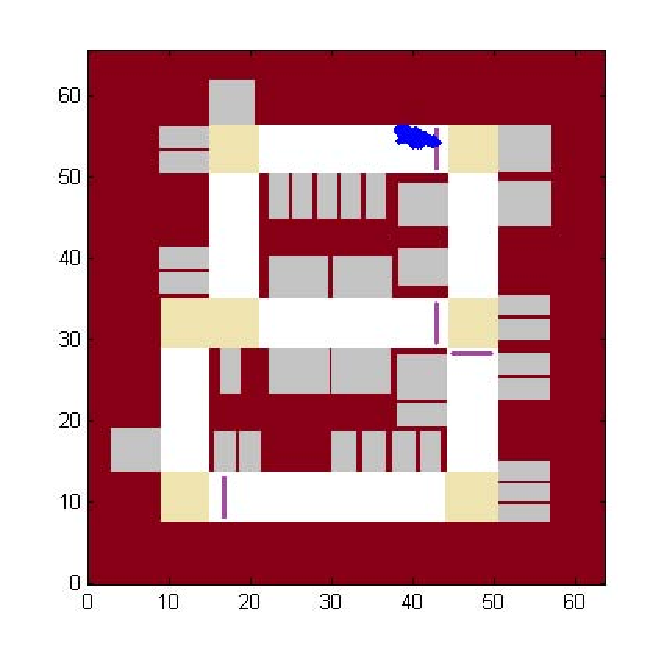
\includegraphics[scale=.3]{fig1-7.pdf}}
  \centerline{(g)}
\end{minipage}
\begin{minipage}{0.32\linewidth}
  \centerline{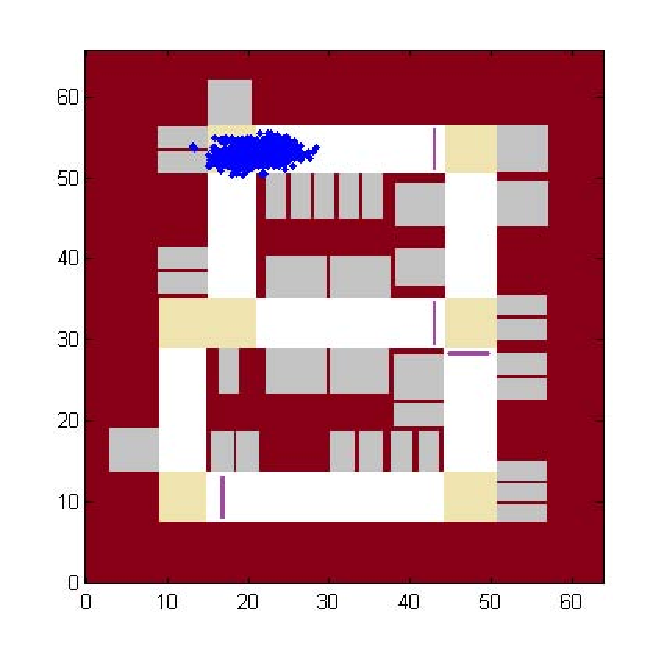
\includegraphics[scale=.3]{fig1-8.pdf}}
  \centerline{(h)}
\end{minipage}
\begin{minipage}{0.32\linewidth}
  \centerline{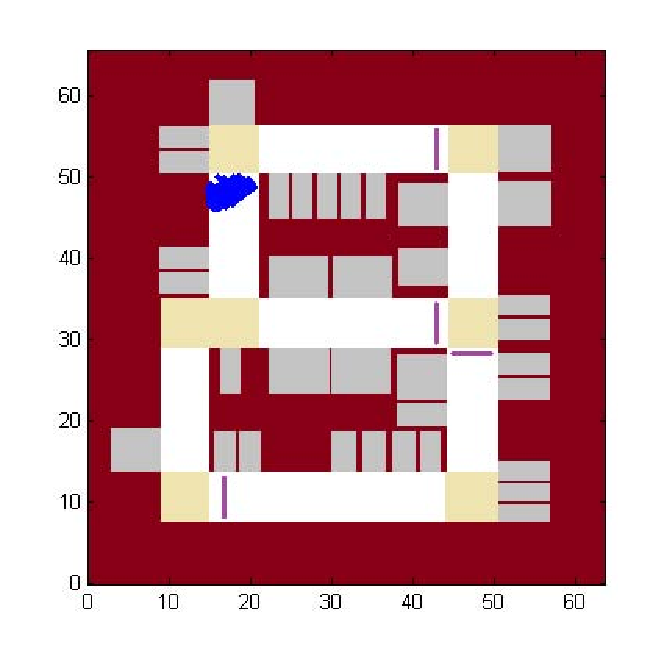
\includegraphics[scale=.3]{fig1-9.pdf}}
  \centerline{(i)}
\end{minipage}
\centering
\begin{minipage}{0.32\linewidth}
  \centerline{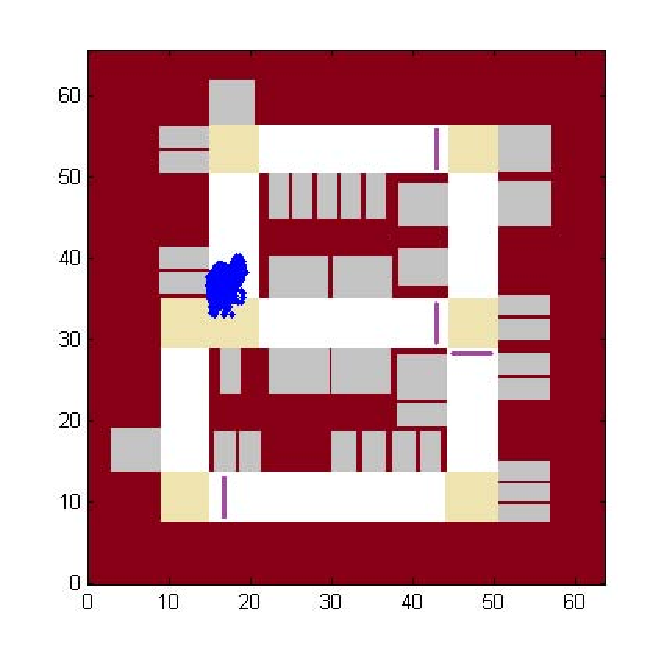
\includegraphics[scale=.3]{fig1-10.pdf}}
  \centerline{(j)}
\end{minipage}
\begin{minipage}{0.32\linewidth}
  \centerline{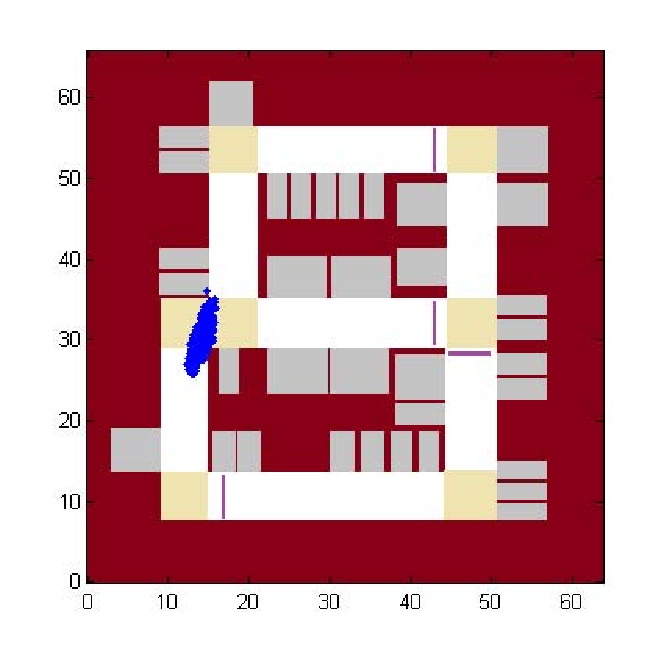
\includegraphics[scale=.3]{fig1-11.pdf}}
  \centerline{(k)}
\end{minipage}
\begin{minipage}{0.32\linewidth}
  \centerline{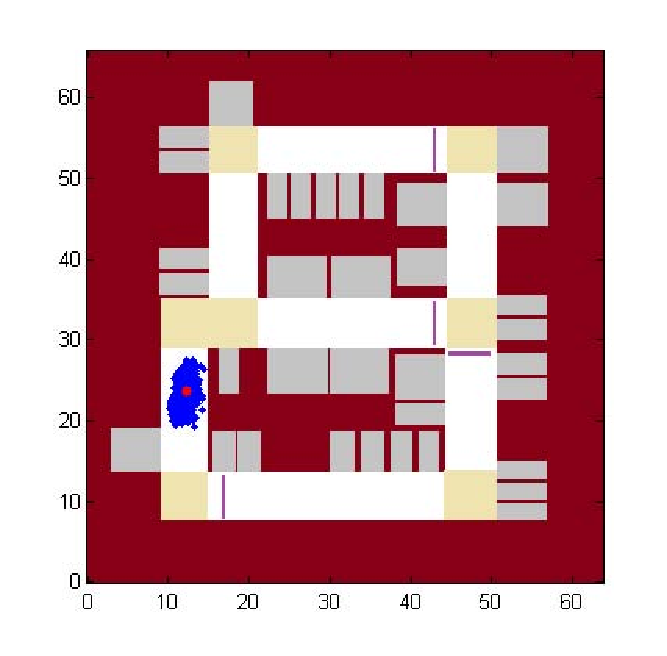
\includegraphics[scale=.3]{fig1-12.pdf}}
  \centerline{(l)}
\end{minipage}
%\end{tabular}
\vspace{5pt}
\caption{Particles over time with initial position and heading direction of the vehicle.}\label{fig_case1}
\end{figure}

\textbf{Experiment with only the initial heading direction of the vehicle.}
Figure \ref{fig_case2} shows the process if the initial position is unknown but the initial heading direction is somehow known (e.g, using compass to find which of the four directions imposed by the parking lot aisles is the most likely one). As shown in Figure \ref{fig_case2}(a), particles are initialized everywhere in the parking lot. As the vehicle starts moving up, constraints imposed by the map filter out many particles that would hit walls when moving up (shown in Figure \ref{fig_case2}(b)). Figure \ref{fig_case2}(c) shows more particles are eliminated when a landmark (i.e., speed bump) is detected, and only those just passing around a speed bump can survive. Figure \ref{fig_case2}(d)(e) show that the detected left turn eliminate many particles and the remaining ones cluster around the corner. Figure \ref{fig_case2}(e) looks similar to Figure \ref{fig_case1}(g), showing that VeLoc succeeds in estimating the state of the vehicle without the initial position. From there the process is similar to the previous one. Figure \ref{fig_case2}(f) shows the final position of all the particles and the average position is shown with a red point, which is very accurate as well. We can also trace back to determine the initial position of the vehicle which is not known at the beginning. % Comparing with the route shown in Figure \ref{fig_route} ), VeLocE gets a very accurate result in localization problem without initial position.


\begin{figure}[htbp]
%\begin{tabular}{cc}
\begin{minipage}{0.32\linewidth}
\centering
  \centerline{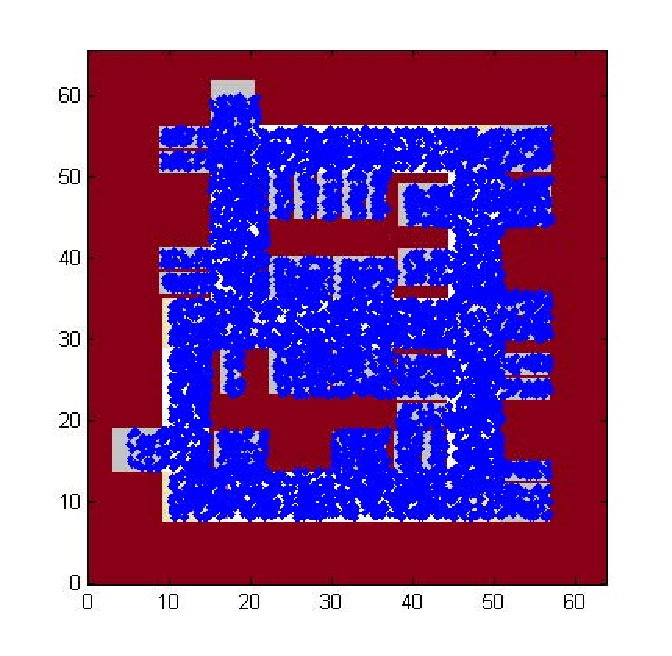
\includegraphics[scale=.3]{fig2-1.pdf}}
  \centerline{(a)}
\end{minipage}
\begin{minipage}{0.32\linewidth}
  \centerline{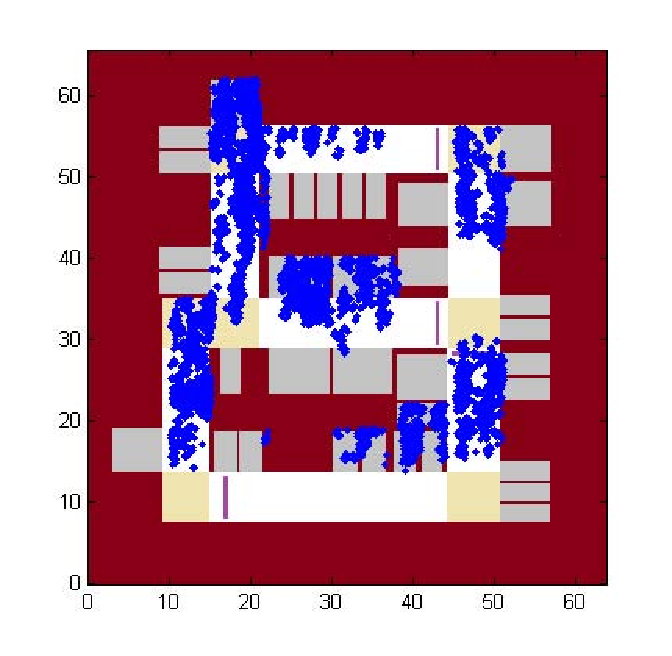
\includegraphics[scale=.3]{fig2-2.pdf}}
  \centerline{(b)}
\end{minipage}
\begin{minipage}{0.32\linewidth}
  \centerline{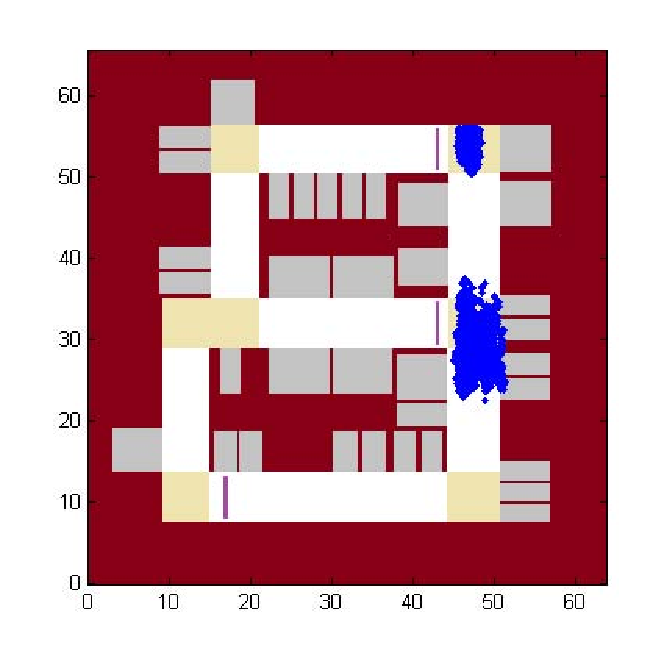
\includegraphics[scale=.3]{fig2-3.pdf}}
  \centerline{(c)}
\end{minipage}
\centering
\begin{minipage}{0.32\linewidth}
  \centerline{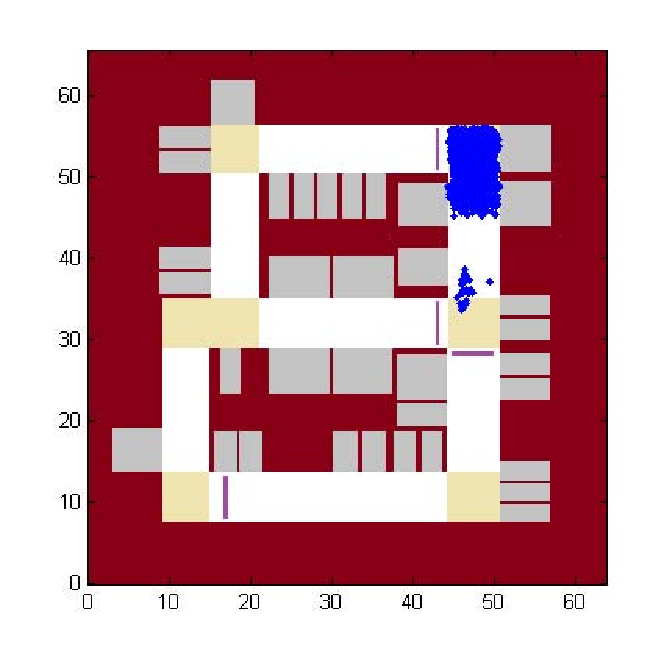
\includegraphics[scale=.3]{fig2-4.pdf}}
  \centerline{(d)}
\end{minipage}
\begin{minipage}{0.32\linewidth}
  \centerline{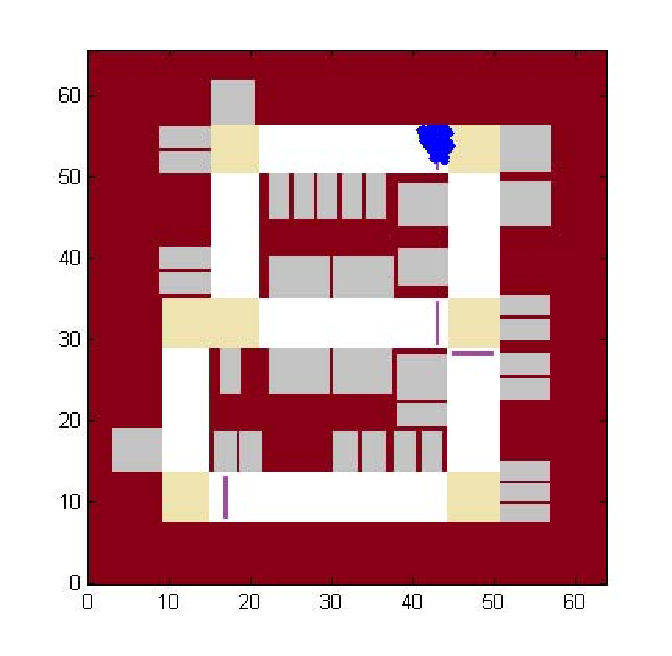
\includegraphics[scale=.3]{fig2-5.pdf}}
  \centerline{(e)}
\end{minipage}
\begin{minipage}{0.32\linewidth}
  \centerline{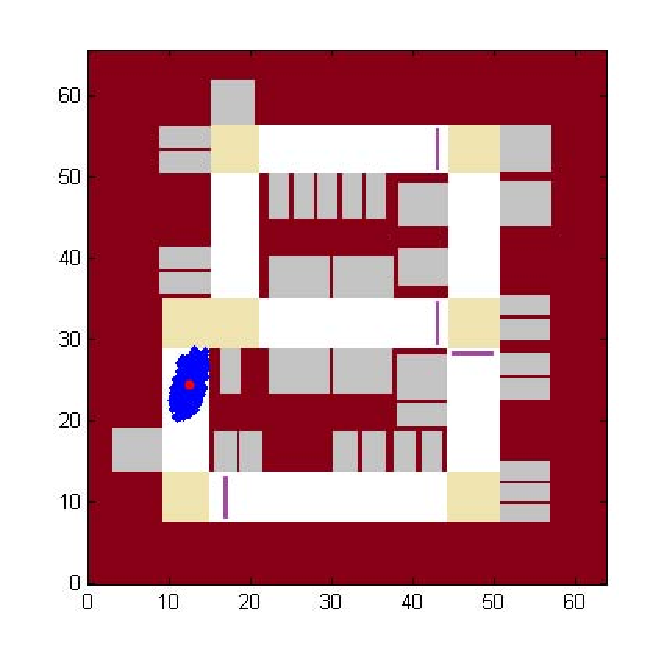
\includegraphics[scale=.3]{fig2-6.pdf}}
  \centerline{(f)}
\end{minipage}
%\end{tabular}
\vspace{5pt}
\caption{Particles over time with only the initial heading of the vehicle.}\label{fig_case2}
\end{figure}

\textbf{Experiment with neither the initial position nor heading direction of the vehicle.}
Figure \ref{fig_case3} shows the results if neither the initial position nor the heading direction is unknown. VeLocE is still able to estimate the true state of the vehicle but it may take a litter longer to converge. As shown in Figure \ref{fig_case3}(a), particles are initialized everywhere in the parking lot. Constraints imposed by the map (i.e., walls) filter out some particles but compared to Figure \ref{fig_case2}(b) they are still widely distributed (shown in Figure \ref{fig_case3}(b)). This is because the lack of heading direction gives more particles the chance to survive. Figure \ref{fig_case3}(c) shows how particles converge quickly when a landmark of speed bump eliminate those without a bump nearby. However, compared to Figure \ref{fig_case2}(c), they are still distributed more widely. In Figure \ref{fig_case3}(d), particles traveling in horizontal directions are eliminated because the vehicle keeps moving upwards, but those traveling vertically become more dispersed. Figure \ref{fig_case3}(e) shows that how a left turn detected remove most of the particles and leaving only close to the true location, the upper right corner. Figure \ref{fig_case3}(f) again shows the final positions of all the particles and their average position shown with a red point. From this example, we can see that VeLocE can produce very accurate results even both the initial position and the heading direction are unknown.

\begin{figure}[htbp]
%\begin{tabular}{cc}
\begin{minipage}{0.32\linewidth}
\centering
  \centerline{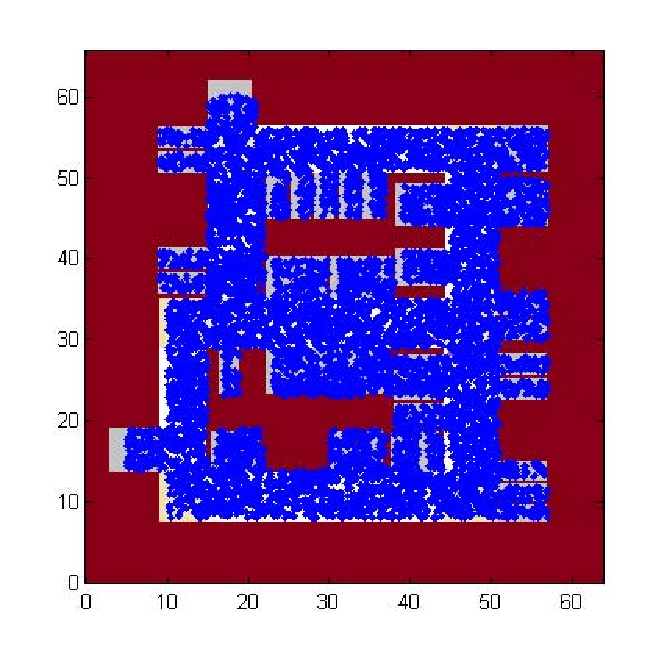
\includegraphics[scale=.3]{fig3-1.pdf}}
  \centerline{(a)}
\end{minipage}
\begin{minipage}{0.32\linewidth}
  \centerline{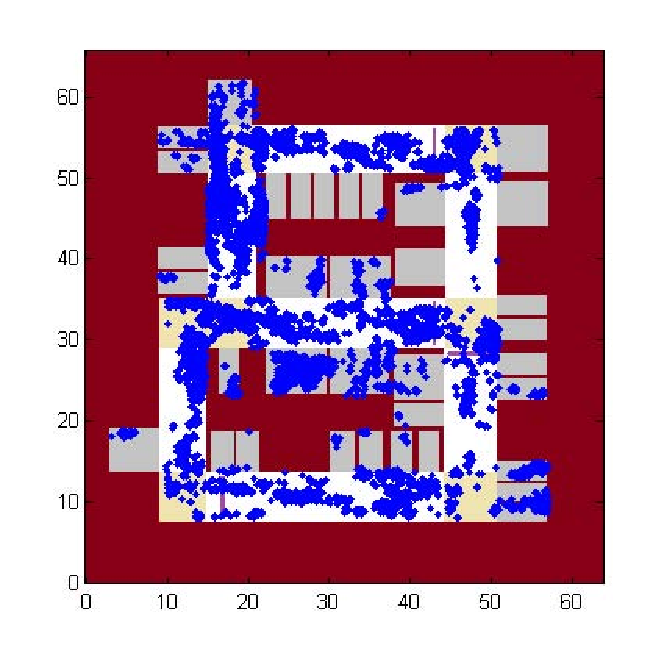
\includegraphics[scale=.3]{fig3-2.pdf}}
  \centerline{(b)}
\end{minipage}
\begin{minipage}{0.32\linewidth}
  \centerline{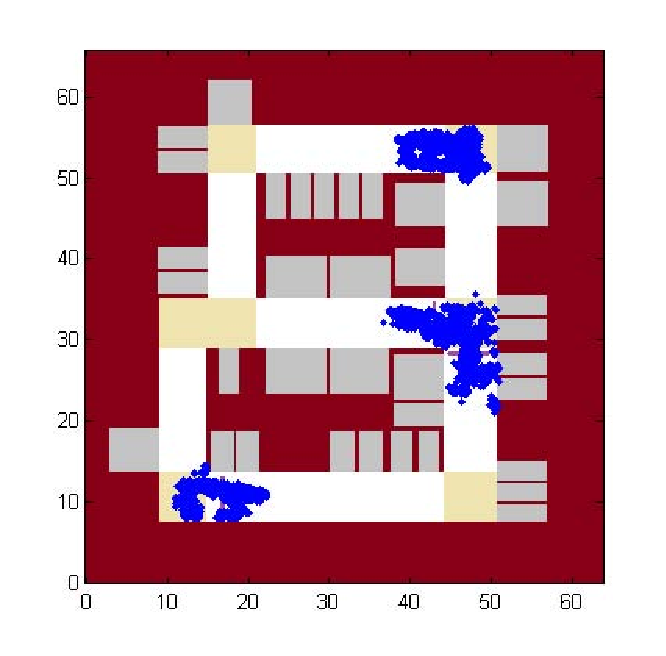
\includegraphics[scale=.3]{fig3-3.pdf}}
  \centerline{(c)}
\end{minipage}
\centering
\begin{minipage}{0.32\linewidth}
  \centerline{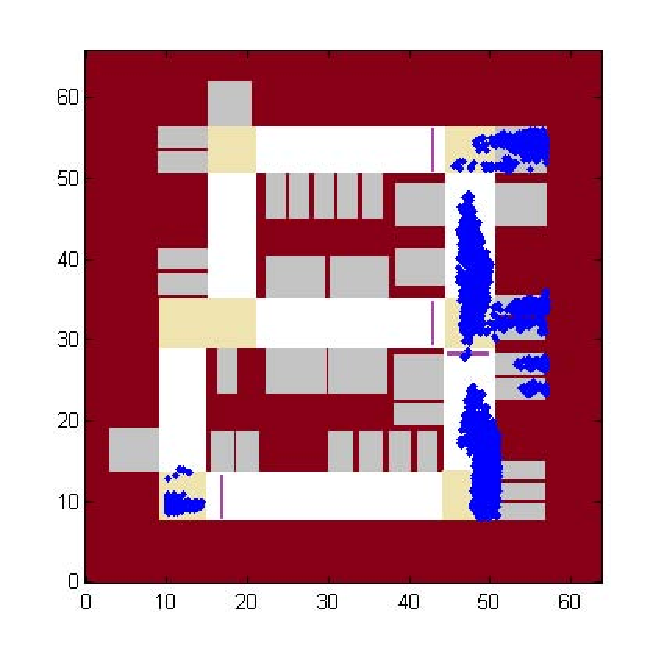
\includegraphics[scale=.3]{fig3-4.pdf}}
  \centerline{(d)}
\end{minipage}
\begin{minipage}{0.32\linewidth}
  \centerline{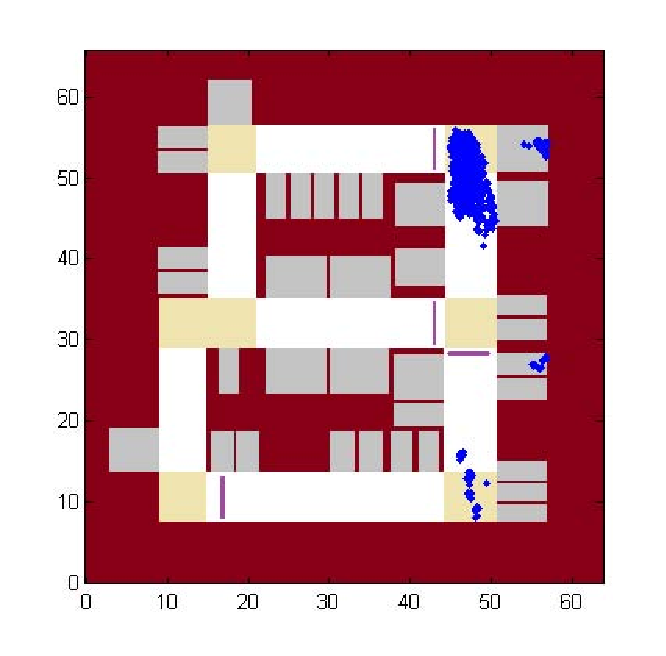
\includegraphics[scale=.3]{fig3-5.pdf}}
  \centerline{(e)}
\end{minipage}
\begin{minipage}{0.32\linewidth}
  \centerline{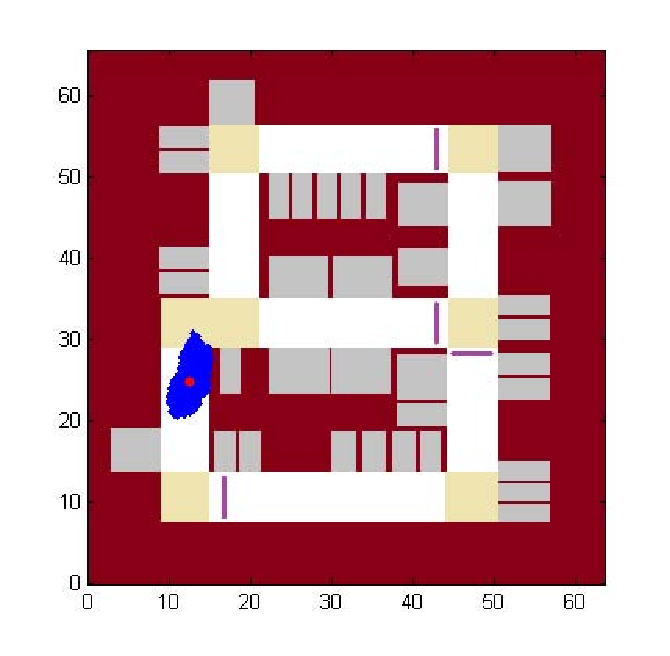
\includegraphics[scale=.3]{fig3-6.pdf}}
  \centerline{(f)}
\end{minipage}
%\end{tabular}
\vspace{5pt}
\caption{Particles over time with neither the initial position or initial heading direction of the vehicle.}\label{fig_case3}
\end{figure}




































\iffalse
In this section we describe how VeLocE uses Augmented Particle Filter (APF) to track the vehicles�� paths as they move in a parking lot. We will first introduce the APF algorithm and then describe the time update and the measurement update, which are the two essential steps in all Bayes Filter based algorithms.\\

Particle filter is an alternative nonparametric implementation of the Bayes filter. The key idea of the particle filter is to represent a distribution by a set of samples drawn from this distribution. In particle filters, the samples of a posterior distribution are called \textit{particles} and are denoted as:
\begin{equation*}\mathcal{X}_t := \boldsymbol{x}_{t}^{[1]},\boldsymbol{x}_{t}^{[2]},...,\boldsymbol{x}_{t}^{[M]}\end{equation*}

Each particle $\boldsymbol{x}_t^{[m]}$(with $1\leq m\leq M$)s a concrete instantiation of the state at time t, that is, a hypothesis as to what the true world state may be at time t. Here M denotes the number of particles in the particle set $\mathcal{X}_t$.\\

\textit{Augmented particles} are novel particles that also incorporate the uncertainty in other aspects such as the direction of the smartphone and the velocity of the vehicle.\\

Just like all other Bayes filter algorithms, APF algorithm constructs the distribution at time t recursively from the distribution one time step earlier. Since beliefs are represented by sets of particles, this means that APF construct the particle set $\mathcal{X}_t$ recursively from the set $\mathcal{X}_{t-1}$.\\

The following is the pseudocode for APF algorithm in VeLocE while $\boldsymbol{u}_t$ and $\boldsymbol{z}_t$ are control and measurement at time t.
\begin{algorithm}[htb]
\caption{$ Augmented\underline{\;}Particle\underline{\;}Filter(\mathcal{X}_{t-1}, \boldsymbol{u}_t, \boldsymbol{z}_t) $}
\begin{algorithmic}[1]
\STATE $\overline{\mathcal{X}}_t = \mathcal{X}_t = \emptyset$
\FOR{$m=1$ to $M$}
\STATE sample $\boldsymbol{x}_{t}^{[m]}\thicksim p(\boldsymbol{x}_t|\boldsymbol{u}_t, \boldsymbol{x}_{t-1}^{[m]})$
\STATE $\overline{\mathcal{X}}_t = \overline{\mathcal{X}}_t \cup \{\boldsymbol{x}_{t}^{[m]}\}$
\ENDFOR
\FOR{$m=1$ to $M$}
\STATE $w_{t}^{[m]} = p(\boldsymbol{z}_t|\boldsymbol{x}_{t}^{[m]})$
\ENDFOR
\FOR{$m=1$ to $M$}
\STATE draw $\boldsymbol{x}_{t}^{[i]}$ from $\overline{\mathcal{X}}_t$ with probability $\varpropto w_{t}^{[i]}$
\STATE $\mathcal{X}_t = \mathcal{X}_t \cup \{\boldsymbol{x}_{t}^{[i]}\}$
\ENDFOR
\RETURN $\mathcal{X}_t$
\end{algorithmic}
\end{algorithm}

\textit{Time update}, which is also known as \textit{control update}, is shown in Lines 2 through 5 while \textit{measurement update} is shown in Lines 6 through 12.\\

During the time update, APF generates a hypothetical state $\boldsymbol{x}_{t}^{[m]}$ for time t based on the particle $\boldsymbol{x}_{t-1}^{[m]}$ and the control $\boldsymbol{u}_t$. The resulting sample is indexed by $m$, indicating that it is generated from the $m$-th particle in $\mathcal{X}_{t-1}$. This step involves sampling from the transition distribution $p(\boldsymbol{x}_t|\boldsymbol{u}_t, \boldsymbol{x}_{t-1}^{[m]})$ which is not always possible for arbitrary distributions.\\

During the measurement update, APF first calculates for each particle $\boldsymbol{x}_{t}^{[m]}$ the so-called importance weights, denoted $w_{t}^{[m]}$. Importance weights are used to incorporate the measurement $\boldsymbol{z}_t$ into the particle set. The importance weight, thus, is the probability of the measurement $\boldsymbol{z}_t$ under the particle $\boldsymbol{x}_{t}^{[m]}$, that is, $w_{t}^{[m]} \propto p(\boldsymbol{z}_t|\boldsymbol{x}_{t}^{[m]})$. The real ``trick'' of the particle filter algorithm occurs in Lines 9 through 12 which implements what is known as \textit{resampling} or \textit{importance resampling}. The algorithm draws with replacement $M$ particles from the temporary Set $\overline{\mathcal{X}}_t$ . The probability of drawing each particle is given by its importance weight. By incorporating the importance weights into the resampling process, the distribution of the particles changes over time.\\

In the rest of this section, we describe the transition distribution, importance weights and resampling method in VeLocE.

\subsubsection{Transition Distribution}
To define the transition distribution in VeLocE, we need first introduce the state of a particle and the control. The state of a particle is a four-dimension vector defined as follows:
\begin{equation*}\langle x, y, \theta, v\rangle\end{equation*}
where $x,y$ are position of the vehicle, $\theta$ is the heading direction of the vehicle and $v$ is the velocity along the y-axis of the vehicle shown in Figure \ref{fig_state}. The control is defined as follows:
\begin{equation*}\langle w, a\rangle\end{equation*}
where $w$ is the rotational velocity along the z-axis of the vehicle and $a$ is the acceleration along the y-axis of the vehicle shown in Figure \ref{fig_state}.

\begin{figure}[htbp]
\centering
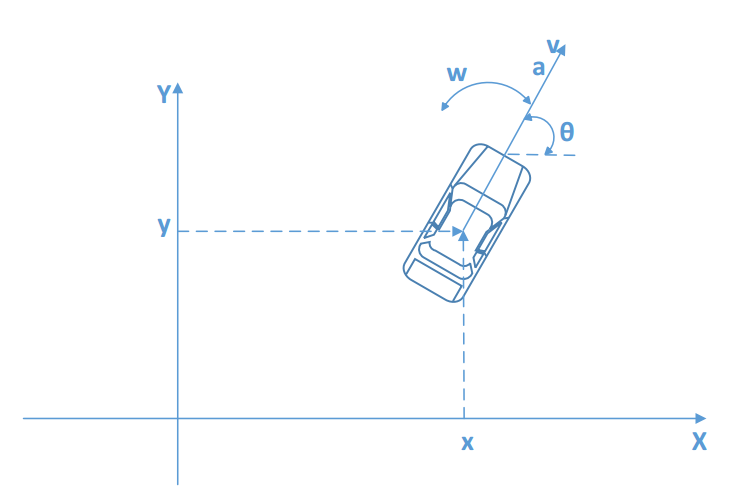
\includegraphics[scale=.46]{state.png}
\caption{State and Control}\label{fig_state}
\end{figure}

We use four-dimension Gaussian distribution
\begin{equation} \mathcal{N}(\boldsymbol{x}_t|\boldsymbol{\mu}_t, \boldsymbol{\Sigma}_t) = \frac{1}{4\pi^2}\frac{1}{|\boldsymbol{\Sigma}_t|^\frac{1}{2}} e^{-\frac{1}{2}(\boldsymbol{x}_t-\boldsymbol{\mu}_t)^{T}\boldsymbol{\Sigma}_t^{-1}(\boldsymbol{x}_t-\boldsymbol{\mu}_t)}\end{equation}
to represent the transition distribution in VeLocE.\\

$\boldsymbol{\mu}_t$ is defined as follows:
\begin{equation}\boldsymbol{\mu_t} = \boldsymbol{G}(\boldsymbol{x}_{t-1}) + \boldsymbol{H}(\boldsymbol{z}_{t})\end{equation}
where
\begin{equation}
\boldsymbol{G}(\boldsymbol{x}_{t-1}) = \boldsymbol{G}(\left(
                                                        \begin{array}{c}
                                                          x_{t-1} \\
                                                          y_{t-1} \\
                                                          \theta_{t-1} \\
                                                          v_{t-1} \\
                                                        \end{array}
                                                      \right))
=\left(
   \begin{array}{c}
     x_{t-1} + v_{t-1}\Delta{t}\cdot\cos{\theta_{t-1}} \\
     y_{t-1} + v_{t-1}\Delta{t}\cdot\sin{\theta_{t-1}} \\
     \theta_{t-1} \\
     v_{t-1} \\
   \end{array}
 \right)
\end{equation}
and
\begin{equation}
\boldsymbol{H}(\boldsymbol{z}_{t}) = \boldsymbol{H}(\left(
                                                      \begin{array}{c}
                                                        w_t \\
                                                        a_t \\
                                                      \end{array}
                                                    \right))
=\left(
   \begin{array}{c}
     0\\
     0\\
     w_t\Delta{t} \\
     a_t\Delta{t} \\
   \end{array}
 \right)
\end{equation}

$\boldsymbol{\Sigma}_t$ is defined as follows:
\begin{equation}
\boldsymbol{\Sigma}_t = \left(
                          \begin{array}{cccc}
                            \sigma_x^2 & 0 & 0 & 0 \\
                            0 & \sigma_y^2 & 0 & 0 \\
                            0 & 0 & \sigma_{\theta}^2 & 0 \\
                            0 & 0 & 0 & \sigma_v^2 \\
                          \end{array}
                        \right)
\end{equation}
where all $\sigma^2$ describe measurement noise.

\subsubsection{Importance Weights}
We define the measurement $\boldsymbol{z}_t$ in VeLocE as follows:
\begin{equation*}\langle road\;anomaly, turning, slope, moving, reachability \rangle\end{equation*}
Every element can take 0 or 1 so that $\boldsymbol{z}_t\in[0,1]^5$. The first three elements are outputs of PD indicating whether a landmark is encountered. The element $moving$ is also one output of PD indicating whether the vehicle is moving. The last element $reachability$ indicates whether the vehicle can reach the current position and obviously is it always 1.\\

To calculate the probability $p(\boldsymbol{z}_t|\boldsymbol{x}_{t}^{[m]})$, we assume that elements of $\boldsymbol{z}_t$ are independent so that:
\begin{equation}
p(\boldsymbol{z}_t|\boldsymbol{x}_{t}^{[m]}) = \prod_{i=1}^{5}{p(z_{ti}|\boldsymbol{x}_{t}^{[m]})}
\end{equation}

As described before, $w_{t}^{[m]} \propto p(\boldsymbol{z}_t|\boldsymbol{x}_{t}^{[m]})$. We can also calculate $w_{t}^{[m]}$ as:
\begin{equation}
w_{t}^{[m]} :=  \prod_{i=1}^{5}{w_{ti}^{[m]}}
\end{equation}
where for $1\leq{i}\leq5$
\begin{equation}
w_{ti}^{[m]} \propto p(z_{ti}|\boldsymbol{x}_{t}^{[m]})
\end{equation}\\

In the rest of this part we will introduce the way to calculate $w_{ti}^{[m]}$ for $1\leq{i}\leq5$.\\

$w_{t1}^{[m]}$ for $road\;anomaly$: Since all the road anomalies are noted on the map, we can calculate for every position $(x,y)$ the closest distance to any road anomalies $dist_{RA}(x,y)$. $w_{t1}^{[m]}$ is defined as follows:

\begin{equation}
w_{t1}^{[m]} = \left\{
                   \begin{array}{ll}
                     1, & \hbox{$road\;anomaly = 0$;} \\
                     \mathcal{N}(dist_{RA}(x_{t1}^{[m]},x_{t2}^{[m]})|0, \sigma_{RA}^2), & \hbox{$road\;anomaly = 1$.}
                   \end{array}
                 \right.
\end{equation}
When a road anomaly is detected, a particle which is closer to a road anomaly noted on the map will have a bigger importance weight.\\

Similarly, $w_{t2}^{[m]}$ and $w_{t2}^{[m]}$ can be defined as follows:
\begin{equation}
w_{t2}^{[m]} = \left\{
                   \begin{array}{ll}
                     1, & \hbox{$turning = 0$;} \\
                     \mathcal{N}(dist_{TU}(x_{t1}^{[m]},x_{t2}^{[m]})|0, \sigma_{TU}^2), & \hbox{$turning = 1$.}
                   \end{array}
                 \right.
\end{equation}

\begin{equation}
w_{t3}^{[m]} = \left\{
                   \begin{array}{ll}
                     1, & \hbox{$slope = 0$;} \\
                     \mathcal{N}(dist_{SL}(x_{t1}^{[m]},x_{t2}^{[m]})|0, \sigma_{SL}^2), & \hbox{$slope = 1$.}
                   \end{array}
                 \right.
\end{equation}

$w_{t4}^{[m]}$ for $moving$: When the vehicle is detected to be immobile, a particle with velocity close to 0 should have a big importance weight. Thus, we define $w_{t4}^{[m]}$ as follows:
\begin{equation}
w_{t4}^{[m]} = \left\{
                   \begin{array}{ll}
                     \mathcal{N}(x_{t4}^{[m]}|0, \sigma_{MV}^2), & \hbox{$moving = 0$;} \\
                     1, & \hbox{$moving = 1$.}
                   \end{array}
                 \right.
\end{equation} \\

$w_{t5}^{[m]}$ for $reachability$: To use the constraints imposed by the map, we give a 0 importance weight to those particles whose positions are noted not able to reach on the map. Assume that $reach(x,y)$ is the information provided by the map to indicate whether the position $(x,y)$ is able to reach. Thus, we define $w_{t5}^{[m]}$ as follows:

\begin{equation}
w_{t5}^{[m]} =
\begin{cases}
1, \hbox{ reach($x_{t1}^{[m]}, x_{t2}^{[m]})=0, reachability=0$;}\\
0, \hbox{ reach($x_{t1}^{[m]}, x_{t2}^{[m]})=0, reachability=1$;}\\
0, \hbox{ reach($x_{t1}^{[m]}, x_{t2}^{[m]})=1, reachability=0$;}\\
1, \hbox{ reach($x_{t1}^{[m]}, x_{t2}^{[m]})=1, reachability=1$;}
\end{cases}
\end{equation}

\subsubsection{Resampling Method}
VeLocE uses Low variance sampler\cite{probabilistic} to fulfill the resampling task. It is worth mentioning that since resampling is most time-consuming part of the algorithm, VeLocE does not perform resampling after every update. VeLocE maintains for each particle an importance weight that is initialized by 1 after resampling and updated multiplicatively untill next resampling. In VelocE, resampling is performed every 10 updates.


\begin{figure*}[htbp]
%\begin{tabular}{cc}
\begin{minipage}{0.32\linewidth}
  \centerline{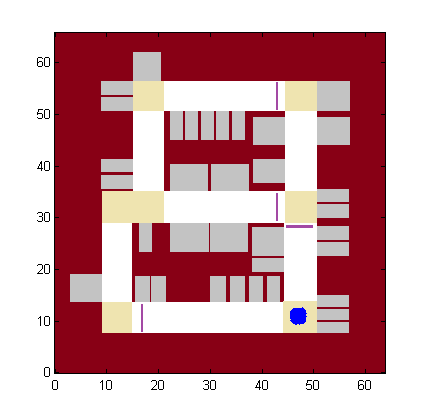
\includegraphics[scale=.3]{fig1-1.png}}
  \centerline{(a)}
\end{minipage}
\begin{minipage}{0.32\linewidth}
  \centerline{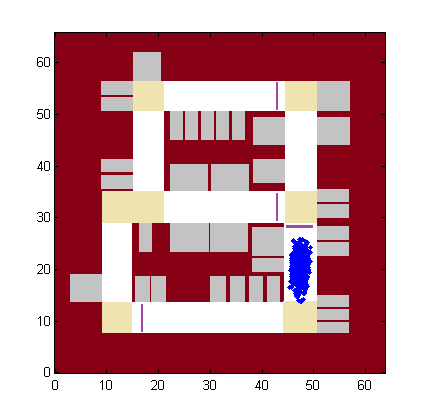
\includegraphics[scale=.3]{fig1-2.png}}
  \centerline{(b)}
\end{minipage}
\begin{minipage}{0.32\linewidth}
  \centerline{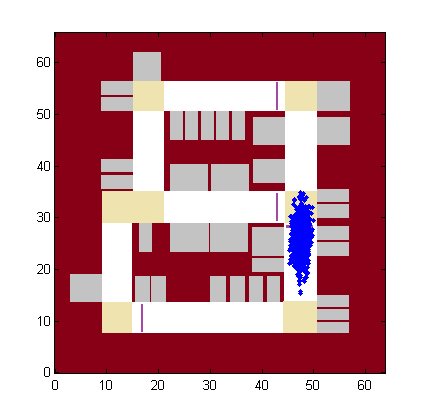
\includegraphics[scale=.3]{fig1-3.png}}
  \centerline{(c)}
\end{minipage}
\begin{minipage}{0.32\linewidth}
  \centerline{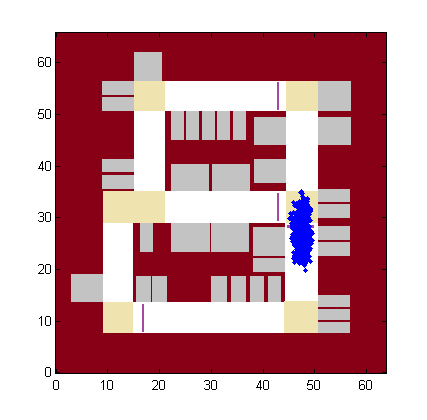
\includegraphics[scale=.3]{fig1-4.png}}
  \centerline{(d)}
\end{minipage}
\begin{minipage}{0.32\linewidth}
  \centerline{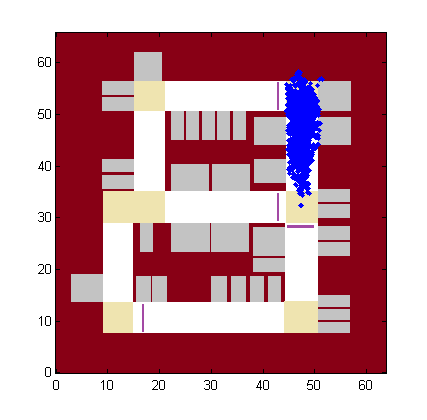
\includegraphics[scale=.3]{fig1-5.png}}
  \centerline{(e)}
\end{minipage}
\begin{minipage}{0.32\linewidth}
  \centerline{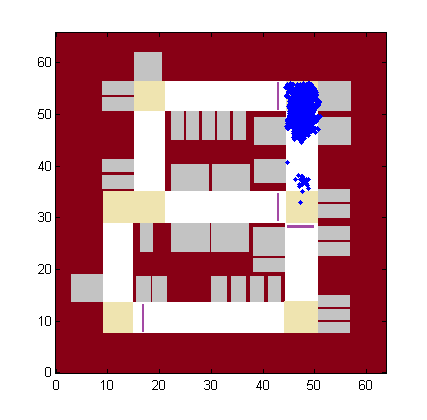
\includegraphics[scale=.3]{fig1-6.png}}
  \centerline{(f)}
\end{minipage}
\begin{minipage}{0.32\linewidth}
  \centerline{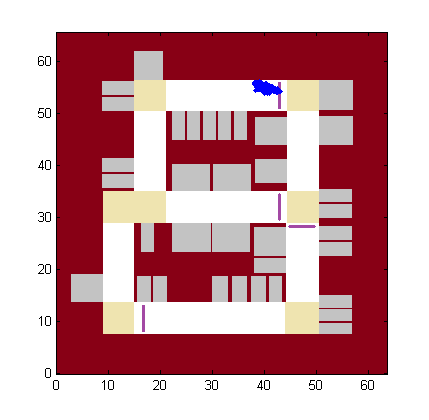
\includegraphics[scale=.3]{fig1-7.png}}
  \centerline{(g)}
\end{minipage}
\begin{minipage}{0.32\linewidth}
  \centerline{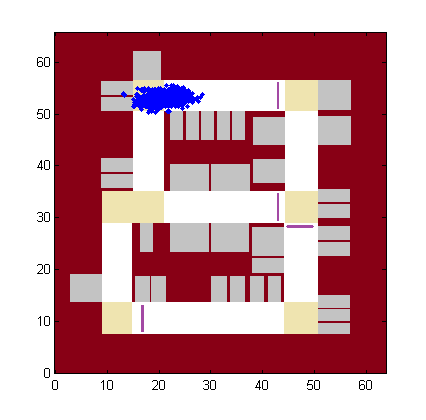
\includegraphics[scale=.3]{fig1-8.png}}
  \centerline{(h)}
\end{minipage}
\begin{minipage}{0.32\linewidth}
  \centerline{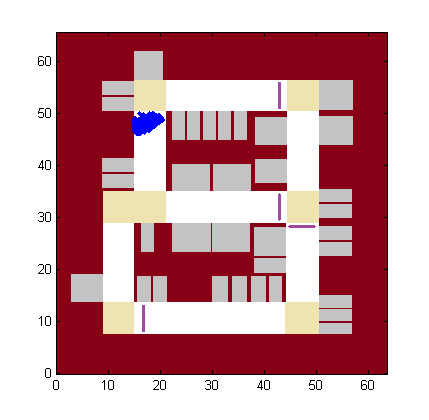
\includegraphics[scale=.3]{fig1-9.png}}
  \centerline{(i)}
\end{minipage}
\begin{minipage}{0.32\linewidth}
  \centerline{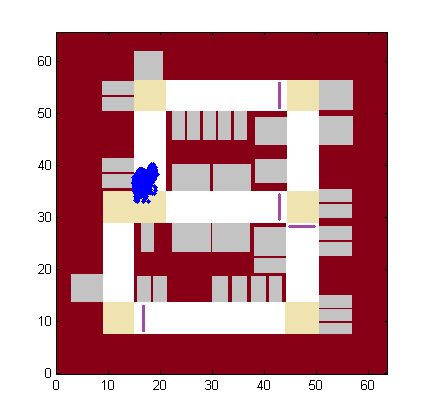
\includegraphics[scale=.3]{fig1-10.png}}
  \centerline{(j)}
\end{minipage}
\begin{minipage}{0.32\linewidth}
  \centerline{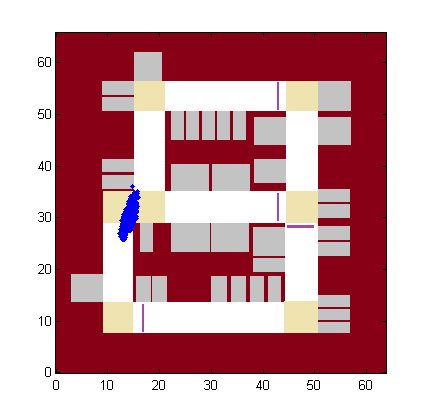
\includegraphics[scale=.3]{fig1-11.png}}
  \centerline{(k)}
\end{minipage}
\begin{minipage}{0.32\linewidth}
  \centerline{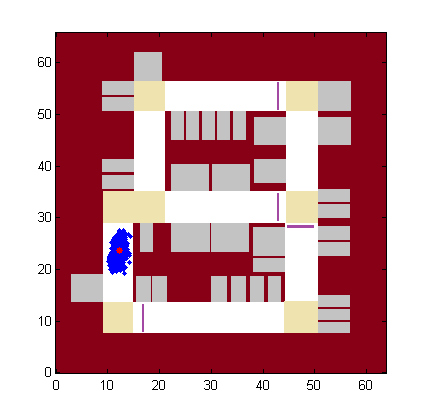
\includegraphics[scale=.3]{fig1-12.png}}
  \centerline{(l)}
\end{minipage}
%\end{tabular}
\caption{Particles over time.}\label{fig_case1}
\end{figure*}

\iffalse
\begin{figure*}[htbp]
%\begin{tabular}{cc}
\begin{minipage}{0.32\linewidth}
  \centerline{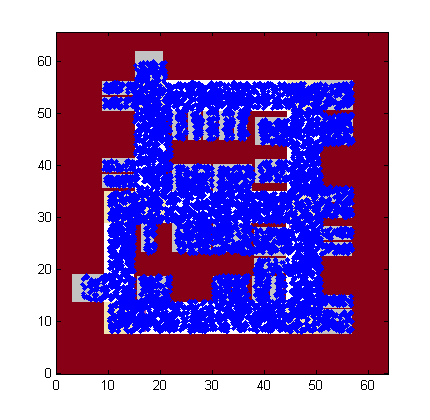
\includegraphics[scale=.3]{fig2-1.png}}
  \centerline{(a)}
\end{minipage}
\begin{minipage}{0.32\linewidth}
  \centerline{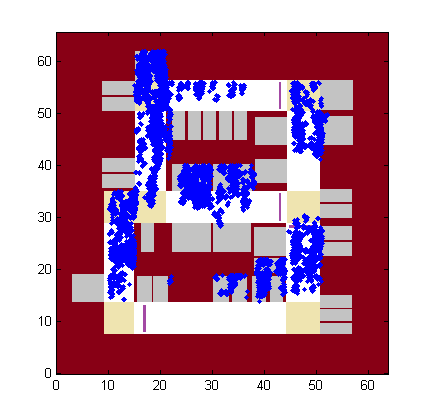
\includegraphics[scale=.3]{fig2-2.png}}
  \centerline{(b)}
\end{minipage}
\begin{minipage}{0.32\linewidth}
  \centerline{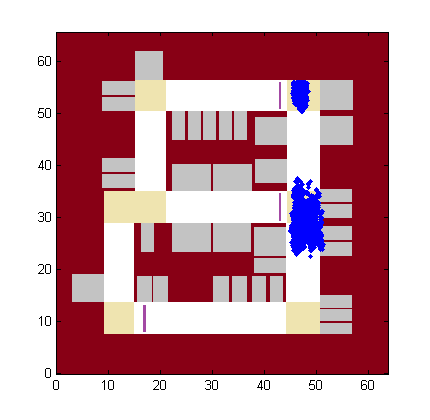
\includegraphics[scale=.3]{fig2-3.png}}
  \centerline{(c)}
\end{minipage}
\begin{minipage}{0.32\linewidth}
  \centerline{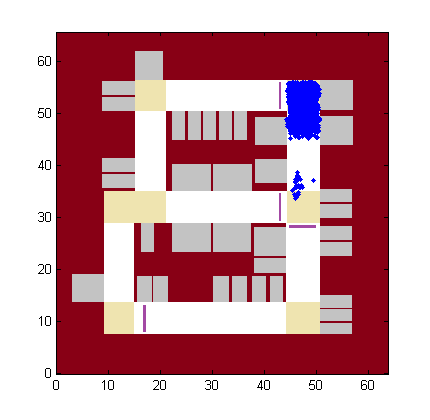
\includegraphics[scale=.3]{fig2-4.png}}
  \centerline{(d)}
\end{minipage}
\begin{minipage}{0.32\linewidth}
  \centerline{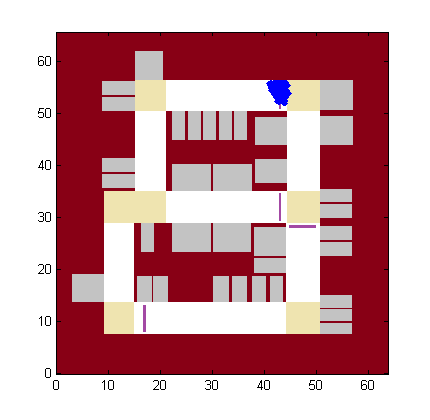
\includegraphics[scale=.3]{fig2-5.png}}
  \centerline{(e)}
\end{minipage}
\begin{minipage}{0.32\linewidth}
  \centerline{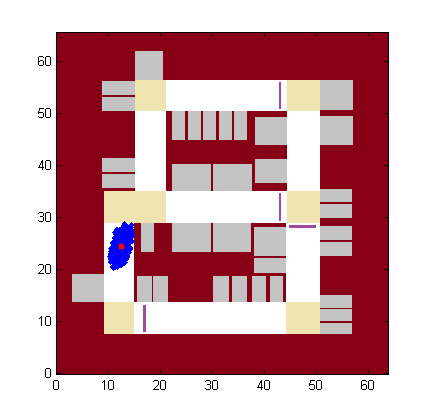
\includegraphics[scale=.3]{fig2-6.png}}
  \centerline{(f)}
\end{minipage}
%\end{tabular}
\caption{Particles over time without the initial position.}\label{fig_case2}
\end{figure*}


\begin{figure*}[htbp]
%\begin{tabular}{cc}
\begin{minipage}{0.32\linewidth}
  \centerline{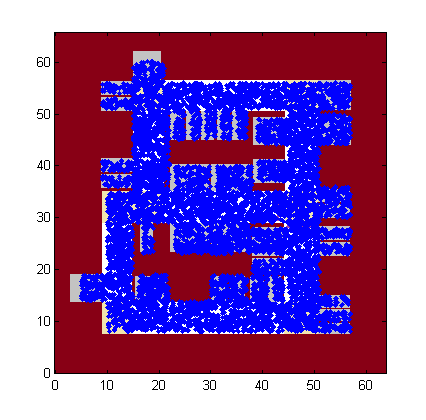
\includegraphics[scale=.3]{fig3-1.png}}
  \centerline{(a)}
\end{minipage}
\begin{minipage}{0.32\linewidth}
  \centerline{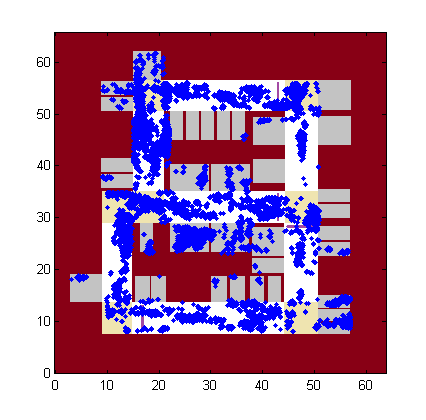
\includegraphics[scale=.3]{fig3-2.png}}
  \centerline{(b)}
\end{minipage}
\begin{minipage}{0.32\linewidth}
  \centerline{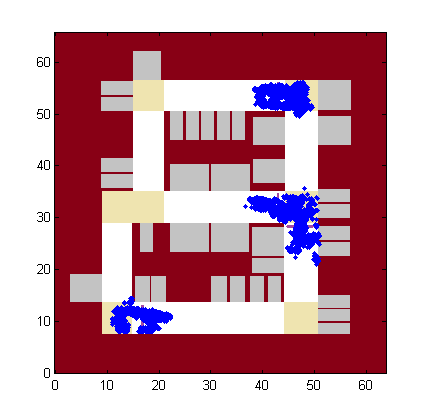
\includegraphics[scale=.3]{fig3-3.png}}
  \centerline{(c)}
\end{minipage}
\begin{minipage}{0.32\linewidth}
  \centerline{\includegraphics[scale=.3]{fig3-4.png}}
  \centerline{(d)}
\end{minipage}
\begin{minipage}{0.32\linewidth}
  \centerline{\includegraphics[scale=.3]{fig3-5.png}}
  \centerline{(e)}
\end{minipage}
\begin{minipage}{0.32\linewidth}
  \centerline{\includegraphics[scale=.3]{fig3-6.png}}
  \centerline{(f)}
\end{minipage}
%\end{tabular}
\caption{Particles over time without the initial position and the initial heading direction.}\label{fig_case3}
\end{figure*}
\fi

In this section, we will show results for the example scenario used in Section \ref{subsec:PD}.\\

We first show results in Figure \ref{fig_case1} which shows the positions of all the particles as time goes by. In this case, the initial state is informed to be somewhere near the entrance of the parking lot. As shown in Figure \ref{fig_case1}(a), all the particles are initialized around the entrance. Figure \ref{fig_case1}(b) shows that particles diverge due to the noise in measurement. Figure \ref{fig_case1}(c)(d) show how speed bumps could make the particles closer. Figure \ref{fig_case1}(e)(f) show how turnings could make the particles closer. Figure \ref{fig_case1}(g) shows all the particles after another turning. Figure \ref{fig_case1}(h)(i) show the ability to estimate the velocity of the vehicle as both particles with velocity being too big or too small will cause the particles reach a wall noted on the map. Figure \ref{fig_case1}(j)(k) show how particles pass through two consecutive turnings. Figure \ref{fig_case1}(l) shows the final position of all the positions and the average position is shown with a red point. Comparing with the route shown in Figure \ref{fig_route}, VeLocE gets a very accurate result in the localization problem.\\

Figure \ref{fig_case2} shows the results if the initial position is unknown but the initial heading direction is somehow known(e.g, using compass and the regularity of heading directions of a vehicle in the parking lot). As shown in Figure \ref{fig_case2}(a), particles are initialized everywhere in the parking lot. While the vehicle is moving, constraints imposed by the map filter out some particles as shown in Figure \ref{fig_case2}(b). Figure \ref{fig_case2}(c) shows how particles converge quickly when a landmark is detected. Figure \ref{fig_case2}(d)(e) show the effect of velocity estimation. Figure \ref{fig_case2}(e) looks similar with Figure \ref{fig_case1}(g) meaning that VeLocE succeed in estimating the state of the vehicle without the initial position. We can also trace back to determine the initial position of the vehicle which is not given at the beginning. Figure \ref{fig_case2}(f) shows the final position of all the positions and the average position is shown with a red point. Comparing with the route shown in Figure \ref{fig_route} ), VeLocE gets a very accurate result in localization problem without initial position.\\

Figure \ref{fig_case3} shows the results if both the initial position and initial heading direction are unknown. VeLocE is still able to estimate the true state of the vehicle but it may take a litter longer time to converge. As shown in Figure \ref{fig_case3}(a), particles are initialized everywhere in the parking lot. Constraints imposed by the map filter out some particles but it still looks bad as shown in Figure \ref{fig_case3}(b). Figure \ref{fig_case3}(c) shows how particles converge quickly when a landmark is detected. However, comparing with Figure \ref{fig_case2}(c), particles converge in more places since the heading direction is unknown. Figure \ref{fig_case3}(d) shows constraints imposed by map filter out some other particles. Figure \ref{fig_case3}(e) shows that particles converge after a second landmark detected. Figure \ref{fig_case3}(f) shows the final position of all the positions and the average position is shown with a red point. Comparing with the route shown in Figure \ref{fig_route} ), VeLocE gets a very accurate result in localization problem without both the initial position and the initial heading direction.

\fi
